\PassOptionsToPackage{unicode=true}{hyperref} % options for packages loaded elsewhere
\PassOptionsToPackage{hyphens}{url}
%
\documentclass[
]{article}
\usepackage{lmodern}
\usepackage{amssymb,amsmath}
\usepackage{ifxetex,ifluatex}
\ifnum 0\ifxetex 1\fi\ifluatex 1\fi=0 % if pdftex
  \usepackage[T1]{fontenc}
  \usepackage[utf8]{inputenc}
  \usepackage{textcomp} % provides euro and other symbols
\else % if luatex or xelatex
  \usepackage{unicode-math}
  \defaultfontfeatures{Scale=MatchLowercase}
  \defaultfontfeatures[\rmfamily]{Ligatures=TeX,Scale=1}
\fi
% use upquote if available, for straight quotes in verbatim environments
\IfFileExists{upquote.sty}{\usepackage{upquote}}{}
\IfFileExists{microtype.sty}{% use microtype if available
  \usepackage[]{microtype}
  \UseMicrotypeSet[protrusion]{basicmath} % disable protrusion for tt fonts
}{}
\makeatletter
\@ifundefined{KOMAClassName}{% if non-KOMA class
  \IfFileExists{parskip.sty}{%
    \usepackage{parskip}
  }{% else
    \setlength{\parindent}{0pt}
    \setlength{\parskip}{6pt plus 2pt minus 1pt}}
}{% if KOMA class
  \KOMAoptions{parskip=half}}
\makeatother
\usepackage{xcolor}
\IfFileExists{xurl.sty}{\usepackage{xurl}}{} % add URL line breaks if available
\IfFileExists{bookmark.sty}{\usepackage{bookmark}}{\usepackage{hyperref}}
\hypersetup{
  pdftitle={ESM 202 Assignment 1},
  pdfauthor={Keene Morrow},
  pdfborder={0 0 0},
  breaklinks=true}
\urlstyle{same}  % don't use monospace font for urls
\usepackage[margin=1in]{geometry}
\usepackage{color}
\usepackage{fancyvrb}
\newcommand{\VerbBar}{|}
\newcommand{\VERB}{\Verb[commandchars=\\\{\}]}
\DefineVerbatimEnvironment{Highlighting}{Verbatim}{commandchars=\\\{\}}
% Add ',fontsize=\small' for more characters per line
\usepackage{framed}
\definecolor{shadecolor}{RGB}{248,248,248}
\newenvironment{Shaded}{\begin{snugshade}}{\end{snugshade}}
\newcommand{\AlertTok}[1]{\textcolor[rgb]{0.94,0.16,0.16}{#1}}
\newcommand{\AnnotationTok}[1]{\textcolor[rgb]{0.56,0.35,0.01}{\textbf{\textit{#1}}}}
\newcommand{\AttributeTok}[1]{\textcolor[rgb]{0.77,0.63,0.00}{#1}}
\newcommand{\BaseNTok}[1]{\textcolor[rgb]{0.00,0.00,0.81}{#1}}
\newcommand{\BuiltInTok}[1]{#1}
\newcommand{\CharTok}[1]{\textcolor[rgb]{0.31,0.60,0.02}{#1}}
\newcommand{\CommentTok}[1]{\textcolor[rgb]{0.56,0.35,0.01}{\textit{#1}}}
\newcommand{\CommentVarTok}[1]{\textcolor[rgb]{0.56,0.35,0.01}{\textbf{\textit{#1}}}}
\newcommand{\ConstantTok}[1]{\textcolor[rgb]{0.00,0.00,0.00}{#1}}
\newcommand{\ControlFlowTok}[1]{\textcolor[rgb]{0.13,0.29,0.53}{\textbf{#1}}}
\newcommand{\DataTypeTok}[1]{\textcolor[rgb]{0.13,0.29,0.53}{#1}}
\newcommand{\DecValTok}[1]{\textcolor[rgb]{0.00,0.00,0.81}{#1}}
\newcommand{\DocumentationTok}[1]{\textcolor[rgb]{0.56,0.35,0.01}{\textbf{\textit{#1}}}}
\newcommand{\ErrorTok}[1]{\textcolor[rgb]{0.64,0.00,0.00}{\textbf{#1}}}
\newcommand{\ExtensionTok}[1]{#1}
\newcommand{\FloatTok}[1]{\textcolor[rgb]{0.00,0.00,0.81}{#1}}
\newcommand{\FunctionTok}[1]{\textcolor[rgb]{0.00,0.00,0.00}{#1}}
\newcommand{\ImportTok}[1]{#1}
\newcommand{\InformationTok}[1]{\textcolor[rgb]{0.56,0.35,0.01}{\textbf{\textit{#1}}}}
\newcommand{\KeywordTok}[1]{\textcolor[rgb]{0.13,0.29,0.53}{\textbf{#1}}}
\newcommand{\NormalTok}[1]{#1}
\newcommand{\OperatorTok}[1]{\textcolor[rgb]{0.81,0.36,0.00}{\textbf{#1}}}
\newcommand{\OtherTok}[1]{\textcolor[rgb]{0.56,0.35,0.01}{#1}}
\newcommand{\PreprocessorTok}[1]{\textcolor[rgb]{0.56,0.35,0.01}{\textit{#1}}}
\newcommand{\RegionMarkerTok}[1]{#1}
\newcommand{\SpecialCharTok}[1]{\textcolor[rgb]{0.00,0.00,0.00}{#1}}
\newcommand{\SpecialStringTok}[1]{\textcolor[rgb]{0.31,0.60,0.02}{#1}}
\newcommand{\StringTok}[1]{\textcolor[rgb]{0.31,0.60,0.02}{#1}}
\newcommand{\VariableTok}[1]{\textcolor[rgb]{0.00,0.00,0.00}{#1}}
\newcommand{\VerbatimStringTok}[1]{\textcolor[rgb]{0.31,0.60,0.02}{#1}}
\newcommand{\WarningTok}[1]{\textcolor[rgb]{0.56,0.35,0.01}{\textbf{\textit{#1}}}}
\usepackage{graphicx,grffile}
\makeatletter
\def\maxwidth{\ifdim\Gin@nat@width>\linewidth\linewidth\else\Gin@nat@width\fi}
\def\maxheight{\ifdim\Gin@nat@height>\textheight\textheight\else\Gin@nat@height\fi}
\makeatother
% Scale images if necessary, so that they will not overflow the page
% margins by default, and it is still possible to overwrite the defaults
% using explicit options in \includegraphics[width, height, ...]{}
\setkeys{Gin}{width=\maxwidth,height=\maxheight,keepaspectratio}
\setlength{\emergencystretch}{3em}  % prevent overfull lines
\providecommand{\tightlist}{%
  \setlength{\itemsep}{0pt}\setlength{\parskip}{0pt}}
\setcounter{secnumdepth}{-2}
% Redefines (sub)paragraphs to behave more like sections
\ifx\paragraph\undefined\else
  \let\oldparagraph\paragraph
  \renewcommand{\paragraph}[1]{\oldparagraph{#1}\mbox{}}
\fi
\ifx\subparagraph\undefined\else
  \let\oldsubparagraph\subparagraph
  \renewcommand{\subparagraph}[1]{\oldsubparagraph{#1}\mbox{}}
\fi

% set default figure placement to htbp
\makeatletter
\def\fps@figure{htbp}
\makeatother

\usepackage{booktabs}
\usepackage{longtable}
\usepackage{array}
\usepackage{multirow}
\usepackage{wrapfig}
\usepackage{float}
\usepackage{colortbl}
\usepackage{pdflscape}
\usepackage{tabu}
\usepackage{threeparttable}
\usepackage{threeparttablex}
\usepackage[normalem]{ulem}
\usepackage{makecell}
\usepackage{xcolor}

\title{ESM 202 Assignment 1}
\author{Keene Morrow}
\date{1/21/2020}

\begin{document}
\maketitle

\begin{table}[H]
\centering
\begin{tabular}{r|l|l|l|l|r}
\hline
\multicolumn{6}{c|}{Chesapeake Bay Contributing Rivers} \\
\cline{1-6}
USGS Site ID & River & River Abbreviation & Location & State & Mean Flow (m3/s)\\
\hline
1578310 & Susquehanna River & SUS & Conowingo & MD & 1145\\
\hline
1646580 & Potomac River & POT & Chain Br & DC & 347\\
\hline
2035000 & James River & NA & Cartersville & VA & 200\\
\hline
1668000 & Rappahannock River & NA & Fredericksburg & VA & 49\\
\hline
2041650 & Appomattox River & NA & Matoaca & VA & 34\\
\hline
1673000 & Pamunkey River & NA & Hanover & VA & 28\\
\hline
1674500 & Mattaponi River & NA & Beulahville & VA & 15\\
\hline
1594440 & Patuxent River & NA & Bowie & MD & 11\\
\hline
1491000 & Choptank River & CHO & Greensboro & MD & 4\\
\hline
\end{tabular}
\end{table}

\hypertarget{mass-balance}{%
\subsubsection{1. Mass Balance}\label{mass-balance}}

\hypertarget{a-calculate-the-percent-contribution-of-each-river-to-the-total-water-flux-into-the-chesapeake-bay.}{%
\paragraph{a) Calculate the percent contribution of each river to the
total water flux into the Chesapeake
Bay.}\label{a-calculate-the-percent-contribution-of-each-river-to-the-total-water-flux-into-the-chesapeake-bay.}}

\begin{Shaded}
\begin{Highlighting}[]
\NormalTok{river_contrib <-}\StringTok{ }\NormalTok{rivers }\OperatorTok
\StringTok{  }\KeywordTok{mutate}\NormalTok{(}\DataTypeTok{pct_contrib =} \KeywordTok{round}\NormalTok{((mean_flow_m3_s }\OperatorTok{/}\StringTok{ }\NormalTok{ch_tot_inflow)}\OperatorTok{*}\DecValTok{100}\NormalTok{, }\DataTypeTok{digits =} \DecValTok{2}\NormalTok{)) }\OperatorTok
\StringTok{  }\KeywordTok{select}\NormalTok{(river, pct_contrib) }\OperatorTok
\StringTok{  }\KeywordTok{rename}\NormalTok{(}\StringTok{"Percent Contribution"}\NormalTok{ =}\StringTok{ }\NormalTok{pct_contrib,}
         \DataTypeTok{River =}\NormalTok{ river)}
\end{Highlighting}
\end{Shaded}

\begin{table}[H]
\centering
\begin{tabular}{l|r}
\hline
\multicolumn{2}{c|}{\makecell[c]{Table 1.\\Percent Contribution to Chesapeake Bay Flux by River}} \\
\cline{1-2}
River & Percent Contribution\\
\hline
Susquehanna River & 62.47\\
\hline
Potomac River & 18.93\\
\hline
James River & 10.91\\
\hline
Rappahannock River & 2.67\\
\hline
Appomattox River & 1.85\\
\hline
Pamunkey River & 1.53\\
\hline
Mattaponi River & 0.82\\
\hline
Patuxent River & 0.60\\
\hline
Choptank River & 0.22\\
\hline
\end{tabular}
\end{table}

\hypertarget{b-considering-the-rivers-as-the-total-inflow-what-is-the-approximate-turnover-time-for-water-in-the-chesapeake-bay-assume-that-tidal-exchange-has-no-net-effect-on-the-total-volume-of-the-chesapeake-bay.}{%
\paragraph{b) Considering the rivers as the total inflow, what is the
approximate turnover time for water in the Chesapeake Bay? Assume that
tidal exchange has no net effect on the total volume of the Chesapeake
Bay.}\label{b-considering-the-rivers-as-the-total-inflow-what-is-the-approximate-turnover-time-for-water-in-the-chesapeake-bay-assume-that-tidal-exchange-has-no-net-effect-on-the-total-volume-of-the-chesapeake-bay.}}

\begin{Shaded}
\begin{Highlighting}[]
\CommentTok{# Chesapeake Bay turnover in seconds}
\NormalTok{ch_turnover <-}\StringTok{ }\NormalTok{ch_tot_V_m }\OperatorTok{/}\StringTok{ }\NormalTok{ch_tot_inflow}

\CommentTok{# Chesapeake Bay turnover in days}
\NormalTok{ch_turn_days <-}\StringTok{ }\NormalTok{ch_turnover }\OperatorTok{/}\StringTok{ }\NormalTok{(}\DecValTok{60} \OperatorTok{^}\StringTok{ }\DecValTok{2} \OperatorTok{*}\StringTok{ }\DecValTok{24}\NormalTok{)}

\CommentTok{# Chesapeake Bay turnover in years}
\NormalTok{ch_turn_yr <-}\StringTok{ }\NormalTok{ch_turn_days }\OperatorTok{/}\StringTok{ }\FloatTok{365.25}
\end{Highlighting}
\end{Shaded}

The turnover time of the Chesapeake Bay is 429.37 days or 1.18 years.

\hypertarget{c-what-is-the-mean-concentration-in-ux3bcgl-of-total-nitrogen-tn-and-total-phosphorus-tp-entering-the-chesapeake-bay-from-each-river-only-sus-pot-and-cho-in-the-1st-quarter-of-2010}{%
\paragraph{c) What is the mean concentration (in μg/L) of total nitrogen
(TN) and total phosphorus (TP) entering the Chesapeake Bay from each
river (only SUS, POT and CHO) in the 1st quarter of
2010?}\label{c-what-is-the-mean-concentration-in-ux3bcgl-of-total-nitrogen-tn-and-total-phosphorus-tp-entering-the-chesapeake-bay-from-each-river-only-sus-pot-and-cho-in-the-1st-quarter-of-2010}}

\begin{Shaded}
\begin{Highlighting}[]
\CommentTok{# Total Phosphorus kg/day, 2010, Quarter 1, in order, SUS, POT, CHO}
\NormalTok{tp_}\DecValTok{2010}\NormalTok{_q1_kg_d <-}\StringTok{ }\KeywordTok{c}\NormalTok{(}\FloatTok{1.6} \OperatorTok{*}\StringTok{ }\DecValTok{7200}\NormalTok{, }\FloatTok{1.4} \OperatorTok{*}\StringTok{ }\DecValTok{4700}\NormalTok{, }\FloatTok{1.5} \OperatorTok{*}\StringTok{ }\DecValTok{40}\NormalTok{)}

\CommentTok{# Total Nitrogen kg/day, 2010, Quarter 1, in order, SUS, POT, CHO}
\NormalTok{tn_}\DecValTok{2010}\NormalTok{_q1_kg_d <-}\StringTok{ }\KeywordTok{c}\NormalTok{(}\FloatTok{1.5} \OperatorTok{*}\StringTok{ }\DecValTok{160000}\NormalTok{, }\FloatTok{1.5} \OperatorTok{*}\StringTok{ }\DecValTok{64000}\NormalTok{, }\FloatTok{1.75} \OperatorTok{*}\StringTok{ }\DecValTok{600}\NormalTok{)}

\NormalTok{rivers_ug_L <-}\StringTok{ }\NormalTok{rivers }\OperatorTok
\StringTok{  }\CommentTok{# only the rivers of interest}
\StringTok{  }\KeywordTok{filter}\NormalTok{(river_abb }\OperatorTok\StringTok{ }\KeywordTok{c}\NormalTok{(}\StringTok{"SUS"}\NormalTok{, }\StringTok{"POT"}\NormalTok{, }\StringTok{"CHO"}\NormalTok{)) }\OperatorTok
\StringTok{  }\CommentTok{# add TP and TN data from above}
\StringTok{  }\KeywordTok{cbind}\NormalTok{(tp_}\DecValTok{2010}\NormalTok{_q1_kg_d,}
\NormalTok{        tn_}\DecValTok{2010}\NormalTok{_q1_kg_d) }\OperatorTok\StringTok{ }
\StringTok{  }\CommentTok{# Conversions}
\StringTok{  }\KeywordTok{mutate}\NormalTok{(}\DataTypeTok{mean_flow_L_s =}\NormalTok{ mean_flow_m3_s }\OperatorTok{*}\StringTok{ }\DecValTok{1000}\NormalTok{,}
         \DataTypeTok{tp_2010_q1_ug_d =}\NormalTok{ tp_}\DecValTok{2010}\NormalTok{_q1_kg_d }\OperatorTok{*}\StringTok{ }\DecValTok{10} \OperatorTok{^}\StringTok{ }\DecValTok{9}\NormalTok{,}
         \DataTypeTok{tn_2010_q1_ug_d =}\NormalTok{ tn_}\DecValTok{2010}\NormalTok{_q1_kg_d }\OperatorTok{*}\StringTok{ }\DecValTok{10} \OperatorTok{^}\StringTok{ }\DecValTok{9}\NormalTok{) }\OperatorTok
\StringTok{  }\KeywordTok{mutate}\NormalTok{(}\DataTypeTok{tp_2010_q1_ug_s =}\NormalTok{ tp_}\DecValTok{2010}\NormalTok{_q1_ug_d }\OperatorTok{/}\StringTok{ }\DecValTok{86400}\NormalTok{,}
         \DataTypeTok{tn_2010_q1_ug_s =}\NormalTok{ tn_}\DecValTok{2010}\NormalTok{_q1_ug_d }\OperatorTok{/}\StringTok{ }\DecValTok{86400}\NormalTok{) }\OperatorTok
\StringTok{  }\CommentTok{# Calculate Mean Concentration of TP and TN in each river}
\StringTok{  }\KeywordTok{mutate}\NormalTok{(}\DataTypeTok{mean_conc_tp_2010_q1_ug_L =}\NormalTok{ tp_}\DecValTok{2010}\NormalTok{_q1_ug_s }\OperatorTok{/}\StringTok{ }\NormalTok{mean_flow_L_s,}
         \DataTypeTok{mean_conc_tn_2010_q1_ug_L =}\NormalTok{ tn_}\DecValTok{2010}\NormalTok{_q1_ug_s }\OperatorTok{/}\StringTok{ }\NormalTok{mean_flow_L_s)}

\CommentTok{# Prep df for table}
\NormalTok{mean_conc_}\DecValTok{2010}\NormalTok{ <-}\StringTok{ }\NormalTok{rivers_ug_L }\OperatorTok
\StringTok{  }\KeywordTok{select}\NormalTok{(river, mean_conc_tp_}\DecValTok{2010}\NormalTok{_q1_ug_L, mean_conc_tn_}\DecValTok{2010}\NormalTok{_q1_ug_L) }\OperatorTok
\StringTok{  }\KeywordTok{mutate}\NormalTok{(}\DataTypeTok{mean_conc_tp_2010_q1_ug_L =} \KeywordTok{round}\NormalTok{(mean_conc_tp_}\DecValTok{2010}\NormalTok{_q1_ug_L, }\DataTypeTok{digits =} \DecValTok{2}\NormalTok{),}
         \DataTypeTok{mean_conc_tn_2010_q1_ug_L=} \KeywordTok{round}\NormalTok{(mean_conc_tn_}\DecValTok{2010}\NormalTok{_q1_ug_L, }\DataTypeTok{digits =} \DecValTok{2}\NormalTok{)) }\OperatorTok\StringTok{ }
\StringTok{  }\KeywordTok{rename}\NormalTok{(}\StringTok{"Total Phosphorus"}\NormalTok{ =}\StringTok{ }\NormalTok{mean_conc_tp_}\DecValTok{2010}\NormalTok{_q1_ug_L,}
         \StringTok{"Total Nitrogen"}\NormalTok{ =}\StringTok{ }\NormalTok{mean_conc_tn_}\DecValTok{2010}\NormalTok{_q1_ug_L,}
         \DataTypeTok{River =}\NormalTok{ river)}
\end{Highlighting}
\end{Shaded}

\begin{table}[H]
\centering
\begin{tabular}{l|r|r}
\hline
\multicolumn{3}{c|}{\makecell[c]{Table 2.\\Mean Concentrations (µg/L) entering the Chesapeake Bay by River\\Quarter 1, 2010}} \\
\cline{1-3}
River & Total Phosphorus & Total Nitrogen\\
\hline
Susquehanna River & 116.45 & 2426.01\\
\hline
Potomac River & 219.47 & 3202.05\\
\hline
Choptank River & 173.61 & 3038.19\\
\hline
\end{tabular}
\end{table}

\hypertarget{d-express-the-concentrations-of-tn-and-tp-also-in-terms-of-molesl-of-n-and-p.}{%
\paragraph{d) Express the concentrations of TN and TP also in terms of
moles/L of N and
P.}\label{d-express-the-concentrations-of-tn-and-tp-also-in-terms-of-molesl-of-n-and-p.}}

\begin{Shaded}
\begin{Highlighting}[]
\NormalTok{N_atomic <-}\StringTok{ }\FloatTok{14.00} \CommentTok{# g / mol}
\NormalTok{P_atomic <-}\StringTok{ }\FloatTok{30.97} \CommentTok{# g / mol}

\NormalTok{N_ug_mol <-}\StringTok{ }\NormalTok{N_atomic }\OperatorTok{*}\StringTok{ }\DecValTok{10} \OperatorTok{^}\StringTok{ }\DecValTok{6} \CommentTok{# ug / mol}
\NormalTok{P_ug_mol <-}\StringTok{ }\NormalTok{P_atomic }\OperatorTok{*}\StringTok{ }\DecValTok{10} \OperatorTok{^}\StringTok{ }\DecValTok{6} \CommentTok{# ug / mol}

\NormalTok{mean_conc_}\DecValTok{2010}\NormalTok{_mol_L <-}\StringTok{ }\NormalTok{rivers_ug_L }\OperatorTok
\StringTok{  }\CommentTok{# Convert ug/L to mol/L}
\StringTok{  }\KeywordTok{mutate}\NormalTok{(}\DataTypeTok{mean_conc_tp_2010_q1_mol_L =}\NormalTok{ mean_conc_tp_}\DecValTok{2010}\NormalTok{_q1_ug_L }\OperatorTok{/}\StringTok{ }\NormalTok{P_ug_mol,}
         \DataTypeTok{mean_conc_tn_2010_q1_mol_L =}\NormalTok{ mean_conc_tn_}\DecValTok{2010}\NormalTok{_q1_ug_L }\OperatorTok{/}\StringTok{ }\NormalTok{N_ug_mol) }\OperatorTok
\StringTok{  }\CommentTok{# Prep for table}
\StringTok{  }\KeywordTok{select}\NormalTok{(river, mean_conc_tp_}\DecValTok{2010}\NormalTok{_q1_mol_L, mean_conc_tn_}\DecValTok{2010}\NormalTok{_q1_mol_L) }\OperatorTok
\StringTok{  }\KeywordTok{mutate}\NormalTok{(}\DataTypeTok{mean_conc_tp_2010_q1_mol_L =} \KeywordTok{formatC}\NormalTok{(mean_conc_tp_}\DecValTok{2010}\NormalTok{_q1_mol_L, }\DataTypeTok{format =} \StringTok{"e"}\NormalTok{, }\DataTypeTok{digits =} \DecValTok{2}\NormalTok{),}
         \DataTypeTok{mean_conc_tn_2010_q1_mol_L=} \KeywordTok{formatC}\NormalTok{(mean_conc_tn_}\DecValTok{2010}\NormalTok{_q1_mol_L, }\DataTypeTok{format=} \StringTok{"e"}\NormalTok{, }\DataTypeTok{digits =} \DecValTok{2}\NormalTok{)) }\OperatorTok
\StringTok{  }\KeywordTok{rename}\NormalTok{(}\StringTok{"Total Phosphorus"}\NormalTok{ =}\StringTok{ }\NormalTok{mean_conc_tp_}\DecValTok{2010}\NormalTok{_q1_mol_L,}
         \StringTok{"Total Nitrogen"}\NormalTok{ =}\StringTok{ }\NormalTok{mean_conc_tn_}\DecValTok{2010}\NormalTok{_q1_mol_L,}
         \DataTypeTok{River =}\NormalTok{ river)}
\end{Highlighting}
\end{Shaded}

\begin{table}[H]
\centering
\begin{tabular}{l|l|l}
\hline
\multicolumn{3}{c|}{\makecell[c]{Table 3.\\Mean Concentrations (mol/L) entering the Chesapeake Bay by River\\Quarter 1, 2010}} \\
\cline{1-3}
River & Total Phosphorus & Total Nitrogen\\
\hline
Susquehanna River & 3.76e-06 & 1.73e-04\\
\hline
Potomac River & 7.09e-06 & 2.29e-04\\
\hline
Choptank River & 5.61e-06 & 2.17e-04\\
\hline
\end{tabular}
\end{table}

\hypertarget{e-how-many-kg-of-tn-and-tp-are-being-discharged-into-the-chesapeake-bay-from-each-river-only-sus-pot-and-cho-in-the-1st-quarter-of-2010}{%
\paragraph{e) How many kg of TN and TP are being discharged into the
Chesapeake Bay from each river (only SUS, POT and CHO) in the 1st
quarter of
2010?}\label{e-how-many-kg-of-tn-and-tp-are-being-discharged-into-the-chesapeake-bay-from-each-river-only-sus-pot-and-cho-in-the-1st-quarter-of-2010}}

\begin{Shaded}
\begin{Highlighting}[]
\NormalTok{t_q1_d <-}\StringTok{ }\DecValTok{31} \OperatorTok{+}\StringTok{ }\CommentTok{# January}
\StringTok{  }\DecValTok{28} \OperatorTok{+}\StringTok{ }\CommentTok{# February}
\StringTok{  }\DecValTok{31} \CommentTok{# March}

\NormalTok{rivers_kg_q1 <-}\StringTok{ }\NormalTok{rivers }\OperatorTok
\StringTok{  }\CommentTok{# only the rivers of interest}
\StringTok{  }\KeywordTok{filter}\NormalTok{(river_abb }\OperatorTok\StringTok{ }\KeywordTok{c}\NormalTok{(}\StringTok{"SUS"}\NormalTok{, }\StringTok{"POT"}\NormalTok{, }\StringTok{"CHO"}\NormalTok{)) }\OperatorTok
\StringTok{  }\CommentTok{# add TP and TN data from above}
\StringTok{  }\KeywordTok{cbind}\NormalTok{(tp_}\DecValTok{2010}\NormalTok{_q1_kg_d,}
\NormalTok{        tn_}\DecValTok{2010}\NormalTok{_q1_kg_d) }\OperatorTok
\StringTok{  }\KeywordTok{mutate}\NormalTok{(}\DataTypeTok{tp_2010_q1_kg_qtr =}\NormalTok{ tp_}\DecValTok{2010}\NormalTok{_q1_kg_d }\OperatorTok{*}\StringTok{ }\NormalTok{t_q1_d,}
         \DataTypeTok{tn_2010_q1_kg_qtr =}\NormalTok{ tn_}\DecValTok{2010}\NormalTok{_q1_kg_d }\OperatorTok{*}\StringTok{ }\NormalTok{t_q1_d) }\OperatorTok
\StringTok{  }\KeywordTok{select}\NormalTok{(river, tp_}\DecValTok{2010}\NormalTok{_q1_kg_qtr, tn_}\DecValTok{2010}\NormalTok{_q1_kg_qtr) }\OperatorTok
\StringTok{  }\KeywordTok{rename}\NormalTok{(}\StringTok{"Total Phosphorus"}\NormalTok{ =}\StringTok{ }\NormalTok{tp_}\DecValTok{2010}\NormalTok{_q1_kg_qtr,}
         \StringTok{"Total Nitrogen"}\NormalTok{ =}\StringTok{ }\NormalTok{tn_}\DecValTok{2010}\NormalTok{_q1_kg_qtr,}
         \DataTypeTok{River =}\NormalTok{ river)}
\end{Highlighting}
\end{Shaded}

\begin{table}[H]
\centering
\begin{tabular}{l|r|r}
\hline
\multicolumn{3}{c|}{\makecell[c]{Table 4.\\Total Contribution (kg) entering the Chesapeake Bay by River \\Quarter 1, 2010}} \\
\cline{1-3}
River & Total Phosphorus & Total Nitrogen\\
\hline
Susquehanna River & 1036800 & 21600000\\
\hline
Potomac River & 592200 & 8640000\\
\hline
Choptank River & 5400 & 94500\\
\hline
\end{tabular}
\end{table}

\hypertarget{f-approximately-what-fraction-of-the-total-mass-of-n-and-p-is-coming-in-as-dissolved-n-dn-or-dissolved-p-dp-in-the-1st-quarter-of-2010}{%
\paragraph{f) Approximately what fraction of the total mass of N and P
is coming in as dissolved N (DN) or dissolved P (DP) in the 1st quarter
of
2010?}\label{f-approximately-what-fraction-of-the-total-mass-of-n-and-p-is-coming-in-as-dissolved-n-dn-or-dissolved-p-dp-in-the-1st-quarter-of-2010}}

\begin{Shaded}
\begin{Highlighting}[]
\CommentTok{# Dissolved Phosphorus kg/day, 2010, Quarter 1, in order, SUS, POT, CHO}
\NormalTok{dp_}\DecValTok{2010}\NormalTok{_q1_kg_d <-}\StringTok{ }\KeywordTok{c}\NormalTok{(}\FloatTok{1.2} \OperatorTok{*}\StringTok{ }\DecValTok{1600}\NormalTok{, }\FloatTok{0.7} \OperatorTok{*}\StringTok{ }\DecValTok{1100}\NormalTok{, }\FloatTok{1.3} \OperatorTok{*}\StringTok{ }\DecValTok{14}\NormalTok{)}

\CommentTok{# Dissolved Nitrogen kg/day, 2010, Quarter 1, in order, SUS, POT, CHO}
\NormalTok{dn_}\DecValTok{2010}\NormalTok{_q1_kg_d <-}\StringTok{ }\KeywordTok{c}\NormalTok{(}\FloatTok{1.4} \OperatorTok{*}\StringTok{ }\DecValTok{140000}\NormalTok{, }\FloatTok{1.5} \OperatorTok{*}\StringTok{ }\DecValTok{48000}\NormalTok{, }\FloatTok{1.7} \OperatorTok{*}\StringTok{ }\DecValTok{540}\NormalTok{)}


\NormalTok{rivers_dis_tot <-}\StringTok{ }\NormalTok{rivers }\OperatorTok
\StringTok{  }\CommentTok{# only the rivers of interest}
\StringTok{  }\KeywordTok{filter}\NormalTok{(river_abb }\OperatorTok\StringTok{ }\KeywordTok{c}\NormalTok{(}\StringTok{"SUS"}\NormalTok{, }\StringTok{"POT"}\NormalTok{, }\StringTok{"CHO"}\NormalTok{)) }\OperatorTok
\StringTok{  }\CommentTok{# add TP, TN, DP, DN data from above}
\StringTok{  }\KeywordTok{cbind}\NormalTok{(dp_}\DecValTok{2010}\NormalTok{_q1_kg_d,}
\NormalTok{        tp_}\DecValTok{2010}\NormalTok{_q1_kg_d) }\OperatorTok
\StringTok{  }\KeywordTok{mutate}\NormalTok{(}\DataTypeTok{dis_tot_P_2010_q1_kg_d =} \KeywordTok{round}\NormalTok{((dp_}\DecValTok{2010}\NormalTok{_q1_kg_d }\OperatorTok{/}\NormalTok{tp_}\DecValTok{2010}\NormalTok{_q1_kg_d), }\DataTypeTok{digits =} \DecValTok{2}\NormalTok{)) }\OperatorTok\StringTok{ }
\StringTok{  }\KeywordTok{cbind}\NormalTok{(dn_}\DecValTok{2010}\NormalTok{_q1_kg_d,}
\NormalTok{        tn_}\DecValTok{2010}\NormalTok{_q1_kg_d) }\OperatorTok
\StringTok{  }\KeywordTok{mutate}\NormalTok{(}\DataTypeTok{dis_tot_N_2010_q1_kg_d =} \KeywordTok{round}\NormalTok{((dn_}\DecValTok{2010}\NormalTok{_q1_kg_d }\OperatorTok{/}\NormalTok{tn_}\DecValTok{2010}\NormalTok{_q1_kg_d), }\DataTypeTok{digits =} \DecValTok{2}\NormalTok{)) }\OperatorTok
\StringTok{  }\KeywordTok{select}\NormalTok{(river, dis_tot_P_}\DecValTok{2010}\NormalTok{_q1_kg_d, dis_tot_N_}\DecValTok{2010}\NormalTok{_q1_kg_d) }\OperatorTok
\StringTok{  }\KeywordTok{rename}\NormalTok{(}\DataTypeTok{River =}\NormalTok{ river,}
         \StringTok{"Nitrogen"}\NormalTok{ =}\StringTok{ }\NormalTok{dis_tot_N_}\DecValTok{2010}\NormalTok{_q1_kg_d,}
         \StringTok{"Phosphorus"}\NormalTok{ =}\StringTok{ }\NormalTok{dis_tot_P_}\DecValTok{2010}\NormalTok{_q1_kg_d)}
\end{Highlighting}
\end{Shaded}

\begin{table}[H]
\centering
\begin{tabular}{l|r|r}
\hline
\multicolumn{3}{c|}{\makecell[c]{Table 5.\\ Contribution of Dissolved Mass to Total Mass entering the Chesapeake Bay by River \\Quarter 1, 2010}} \\
\cline{1-3}
River & Phosphorus & Nitrogen\\
\hline
Susquehanna River & 0.17 & 0.82\\
\hline
Potomac River & 0.12 & 0.75\\
\hline
Choptank River & 0.30 & 0.87\\
\hline
\end{tabular}
\end{table}

\hypertarget{g-calculate-the-total-massday-of-suspended-sediments-being-added-to-the-chesapeake-bay-during-the-1st-quarter-of-2010-by-each-river.}{%
\paragraph{g) Calculate the total mass/day of suspended sediments being
added to the Chesapeake Bay during the 1st quarter of 2010 by each
river.}\label{g-calculate-the-total-massday-of-suspended-sediments-being-added-to-the-chesapeake-bay-during-the-1st-quarter-of-2010-by-each-river.}}

\begin{Shaded}
\begin{Highlighting}[]
\NormalTok{susp_solids <-}\StringTok{ }\KeywordTok{c}\NormalTok{(}\FloatTok{2.2} \OperatorTok{*}\StringTok{ }\DecValTok{4300000}\NormalTok{, }\FloatTok{1.75} \OperatorTok{*}\StringTok{ }\DecValTok{4100000}\NormalTok{, }\FloatTok{1.8} \OperatorTok{*}\StringTok{ }\DecValTok{7100}\NormalTok{)}

\NormalTok{rivers_solids <-}\StringTok{ }\NormalTok{rivers }\OperatorTok
\StringTok{  }\CommentTok{# only the rivers of interest}
\StringTok{  }\KeywordTok{filter}\NormalTok{(river_abb }\OperatorTok\StringTok{ }\KeywordTok{c}\NormalTok{(}\StringTok{"SUS"}\NormalTok{, }\StringTok{"POT"}\NormalTok{, }\StringTok{"CHO"}\NormalTok{)) }\OperatorTok
\StringTok{  }\CommentTok{# add TP, TN, DP, DN data from above}
\StringTok{  }\KeywordTok{cbind}\NormalTok{(susp_solids) }\OperatorTok
\StringTok{  }\KeywordTok{select}\NormalTok{(river, susp_solids) }\OperatorTok
\StringTok{  }\KeywordTok{rename}\NormalTok{(}\DataTypeTok{River =}\NormalTok{ river,}
         \StringTok{"Suspended Solids"}\NormalTok{ =}\StringTok{ }\NormalTok{susp_solids)}
\end{Highlighting}
\end{Shaded}

\begin{table}[H]
\centering
\begin{tabular}{l|r}
\hline
\multicolumn{2}{c|}{\makecell[c]{Table 6.\\ Contribution of Suspended Solids (kg/day) to the Chesapeake Bay by River \\Quarter 1, 2010}} \\
\cline{1-2}
River & Suspended Solids\\
\hline
Susquehanna River & 9460000\\
\hline
Potomac River & 7175000\\
\hline
Choptank River & 12780\\
\hline
\end{tabular}
\end{table}

\hypertarget{water-quality-consider-only-the-sus-pot-and-cho-or-as-indicated}{%
\subsubsection{2. Water quality (consider only the SUS, POT and CHO or
as
indicated)}\label{water-quality-consider-only-the-sus-pot-and-cho-or-as-indicated}}

\hypertarget{a-given-the-molar-ratio-of-100161-cnp-which-nutrient-would-be-limiting-in-each-river-during-the-1st-quarter-of-2010}{%
\paragraph{a) Given the molar ratio of 100:16:1 {[}C:N:P{]}, which
nutrient would be limiting in each river during the 1st quarter of
2010?}\label{a-given-the-molar-ratio-of-100161-cnp-which-nutrient-would-be-limiting-in-each-river-during-the-1st-quarter-of-2010}}

\begin{Shaded}
\begin{Highlighting}[]
\NormalTok{wq_limitation <-}\StringTok{ }\NormalTok{rivers_ug_L }\OperatorTok
\StringTok{  }\CommentTok{# Convert ug/L to mol/L}
\StringTok{  }\KeywordTok{mutate}\NormalTok{(}\DataTypeTok{mean_conc_tp_2010_q1_mol_L =}\NormalTok{ mean_conc_tp_}\DecValTok{2010}\NormalTok{_q1_ug_L }\OperatorTok{/}\StringTok{ }\NormalTok{P_ug_mol,}
         \DataTypeTok{mean_conc_tn_2010_q1_mol_L =}\NormalTok{ mean_conc_tn_}\DecValTok{2010}\NormalTok{_q1_ug_L }\OperatorTok{/}\StringTok{ }\NormalTok{N_ug_mol) }\OperatorTok
\StringTok{  }\KeywordTok{mutate}\NormalTok{(}\DataTypeTok{ratio_N_P =}\NormalTok{ mean_conc_tn_}\DecValTok{2010}\NormalTok{_q1_mol_L }\OperatorTok{/}\StringTok{ }\NormalTok{mean_conc_tp_}\DecValTok{2010}\NormalTok{_q1_mol_L) }\OperatorTok
\StringTok{  }\KeywordTok{mutate}\NormalTok{(}\DataTypeTok{limited =} \KeywordTok{ifelse}\NormalTok{(ratio_N_P }\OperatorTok{<}\StringTok{ }\DecValTok{10}\NormalTok{, }\StringTok{"Nitrogen"}\NormalTok{, }\KeywordTok{ifelse}\NormalTok{(ratio_N_P }\OperatorTok{>}\DecValTok{30}\NormalTok{, }\StringTok{"Phosphorus"}\NormalTok{, }\StringTok{"Not Limited"}\NormalTok{))) }\OperatorTok
\StringTok{  }\KeywordTok{select}\NormalTok{(river, limited) }\OperatorTok
\StringTok{  }\KeywordTok{rename}\NormalTok{(}\DataTypeTok{River =}\NormalTok{ river,}
         \StringTok{"Limited by"}\NormalTok{ =}\StringTok{ }\NormalTok{limited)}
\end{Highlighting}
\end{Shaded}

\begin{table}[H]
\centering
\begin{tabular}{l|l}
\hline
\multicolumn{2}{c|}{\makecell[c]{Table 7.\\ Limiting Nutrients\\Quarter 1, 2010}} \\
\cline{1-2}
River & Limited by\\
\hline
Susquehanna River & Phosphorus\\
\hline
Potomac River & Phosphorus\\
\hline
Choptank River & Phosphorus\\
\hline
\end{tabular}
\end{table}

\hypertarget{b-given-the-molar-ratio-of-100161-cnp-and-given-the-molar-ratio-of-cho-for-biomass-as-121-is-the-dissolved-nitrogen-during-the-1st-quarter-of-2012-likely-to-deplete-oxygen-in-the-choptank-river-assume-the-dissolved-oxygen-is-4.5-mgl-in-the-receiving-water-at-the-point-of-discharge.}{%
\paragraph{b) Given the molar ratio of 100:16:1 {[}C:N:P{]} and given
the molar ratio of C:H:O for biomass as 1:2:1, is the dissolved nitrogen
during the 1st quarter of 2012 likely to deplete oxygen in the Choptank
River? Assume the dissolved oxygen is 4.5 mg/L in the receiving water at
the point of
discharge.}\label{b-given-the-molar-ratio-of-100161-cnp-and-given-the-molar-ratio-of-cho-for-biomass-as-121-is-the-dissolved-nitrogen-during-the-1st-quarter-of-2012-likely-to-deplete-oxygen-in-the-choptank-river-assume-the-dissolved-oxygen-is-4.5-mgl-in-the-receiving-water-at-the-point-of-discharge.}}

\begin{Shaded}
\begin{Highlighting}[]
\NormalTok{DO_mg_L <-}\StringTok{ }\FloatTok{4.5} \CommentTok{# mg/L}
\NormalTok{O_atomic <-}\StringTok{ }\DecValTok{16} \CommentTok{# g / mol}

\NormalTok{DO_mol_L <-}\StringTok{ }\NormalTok{(DO_mg_L }\OperatorTok{/}\StringTok{ }\DecValTok{1000}\NormalTok{) }\OperatorTok{/}\StringTok{ }\DecValTok{16}

\NormalTok{dn_cho_mol_L <-}\StringTok{ }\NormalTok{(rivers_ug_L}\OperatorTok{$}\NormalTok{mean_conc_tn_}\DecValTok{2010}\NormalTok{_q1_ug_L[}\DecValTok{3}\NormalTok{] }\OperatorTok{*}\StringTok{ }\NormalTok{rivers_dis_tot}\OperatorTok{$}\NormalTok{Nitrogen[}\DecValTok{3}\NormalTok{]) }\OperatorTok{/}\StringTok{ }\NormalTok{N_ug_mol}

\NormalTok{dn_cho_mg <-}\StringTok{ }\NormalTok{rivers_ug_L}\OperatorTok{$}\NormalTok{mean_conc_tn_}\DecValTok{2010}\NormalTok{_q1_ug_L[}\DecValTok{3}\NormalTok{] }\OperatorTok{/}\StringTok{ }\DecValTok{1000}

\NormalTok{ratio_dn_DO_cho <-}\StringTok{ }\NormalTok{dn_cho_mol_L }\OperatorTok{/}\StringTok{ }\NormalTok{DO_mol_L}

\NormalTok{ratio_df_el <-}\StringTok{ }\KeywordTok{c}\NormalTok{(}\StringTok{"C"}\NormalTok{, }\StringTok{"N"}\NormalTok{, }\StringTok{"P"}\NormalTok{, }\StringTok{"H"}\NormalTok{, }\StringTok{"O"}\NormalTok{)}
\NormalTok{ratio_df_num <-}\StringTok{ }\KeywordTok{c}\NormalTok{(}\DecValTok{100}\NormalTok{, }\DecValTok{16}\NormalTok{, }\DecValTok{1}\NormalTok{, }\DecValTok{200}\NormalTok{, }\DecValTok{100}\NormalTok{)}
\NormalTok{ratio_cho_DO <-}\StringTok{ }\KeywordTok{c}\NormalTok{(}\StringTok{""}\NormalTok{, }\StringTok{""}\NormalTok{, }\StringTok{""}\NormalTok{, }\StringTok{""}\NormalTok{, DO_mol_L)}
\NormalTok{ratio_cho_DN <-}\StringTok{ }\KeywordTok{c}\NormalTok{(}\StringTok{""}\NormalTok{, dn_cho_mol_L, }\StringTok{""}\NormalTok{, }\StringTok{""}\NormalTok{, }\StringTok{""}\NormalTok{)}

\NormalTok{ratio <-}\StringTok{ }\KeywordTok{as.data.frame}\NormalTok{(ratio_df_el) }\OperatorTok
\StringTok{  }\KeywordTok{cbind}\NormalTok{(ratio_df_num) }\OperatorTok
\StringTok{  }\KeywordTok{mutate}\NormalTok{(}\DataTypeTok{DO_ratio =}\NormalTok{ ratio_df_num }\OperatorTok{/}\StringTok{ }\DecValTok{100}\NormalTok{,}
         \DataTypeTok{DN_ratio =}\NormalTok{ ratio_df_num }\OperatorTok{/}\StringTok{ }\DecValTok{16}\NormalTok{) }\OperatorTok
\StringTok{  }\KeywordTok{mutate}\NormalTok{(}\DataTypeTok{DO_level =}\NormalTok{ DO_ratio }\OperatorTok{*}\StringTok{ }\NormalTok{DO_mol_L,}
         \DataTypeTok{DN_level =}\NormalTok{ DN_ratio }\OperatorTok{*}\StringTok{ }\NormalTok{dn_cho_mol_L) }\OperatorTok
\StringTok{  }\KeywordTok{rename}\NormalTok{(}\DataTypeTok{element =}\NormalTok{ ratio_df_el,}
         \DataTypeTok{std_ratio =}\NormalTok{ ratio_df_num)}
\end{Highlighting}
\end{Shaded}

The maximum dissolved nitrogen level that would not deplete dissolved
oxygen at \ensuremath{2.8125\times 10^{-4}} mol/L is mol/L. The actual
level of dissolved nitrogen in the Choptank River in the first quarter
of 2012 was \ensuremath{1.8880208\times 10^{-4}} mol/L. Thus, it is
expected that dissolved oxygen would be completely depleted.

\hypertarget{c-free-space}{%
\paragraph{c) Free Space}\label{c-free-space}}

\hypertarget{d-given-the-concentrations-of-tn-and-tp-how-would-you-classify-the-eutrophication-potential-of-each-of-the-three-rivers-in-terms-in-the-chesapeake-bay-in-1980-and-2010}{%
\paragraph{d) Given the concentrations of TN and TP, how would you
classify the eutrophication potential of each of the three rivers in
terms in the Chesapeake Bay in 1980 and
2010?}\label{d-given-the-concentrations-of-tn-and-tp-how-would-you-classify-the-eutrophication-potential-of-each-of-the-three-rivers-in-terms-in-the-chesapeake-bay-in-1980-and-2010}}

\begin{Shaded}
\begin{Highlighting}[]
\CommentTok{# Total Phosphorus kg/day, 1980, Quarter 1, in order, SUS, POT, CHO}
\NormalTok{tp_}\DecValTok{1980}\NormalTok{_q1_kg_d <-}\StringTok{ }\KeywordTok{c}\NormalTok{(}\FloatTok{2.0} \OperatorTok{*}\StringTok{ }\DecValTok{7200}\NormalTok{, }\FloatTok{2.0} \OperatorTok{*}\StringTok{ }\DecValTok{4700}\NormalTok{, }\FloatTok{1.3} \OperatorTok{*}\StringTok{ }\DecValTok{40}\NormalTok{)}

\CommentTok{# Total Nitrogen kg/day, 1980, Quarter 1, in order, SUS, POT, CHO}
\NormalTok{tn_}\DecValTok{1980}\NormalTok{_q1_kg_d <-}\StringTok{ }\KeywordTok{c}\NormalTok{(}\FloatTok{1.6} \OperatorTok{*}\StringTok{ }\DecValTok{160000}\NormalTok{, }\FloatTok{1.75} \OperatorTok{*}\StringTok{ }\DecValTok{64000}\NormalTok{, }\FloatTok{1.5} \OperatorTok{*}\StringTok{ }\DecValTok{600}\NormalTok{)}


\NormalTok{eutrophication <-}\StringTok{ }\NormalTok{rivers }\OperatorTok
\StringTok{  }\CommentTok{# only the rivers of interest}
\StringTok{  }\KeywordTok{filter}\NormalTok{(river_abb }\OperatorTok\StringTok{ }\KeywordTok{c}\NormalTok{(}\StringTok{"SUS"}\NormalTok{, }\StringTok{"POT"}\NormalTok{, }\StringTok{"CHO"}\NormalTok{)) }\OperatorTok
\StringTok{  }\CommentTok{# add TP and TN data from above}
\StringTok{  }\KeywordTok{cbind}\NormalTok{(tp_}\DecValTok{1980}\NormalTok{_q1_kg_d,}
\NormalTok{        tn_}\DecValTok{1980}\NormalTok{_q1_kg_d,}
\NormalTok{        tp_}\DecValTok{2010}\NormalTok{_q1_kg_d,}
\NormalTok{        tn_}\DecValTok{2010}\NormalTok{_q1_kg_d) }\OperatorTok\StringTok{ }
\StringTok{  }\CommentTok{# Conversions}
\StringTok{  }\KeywordTok{mutate}\NormalTok{(}\DataTypeTok{mean_flow_L_s =}\NormalTok{ mean_flow_m3_s }\OperatorTok{*}\StringTok{ }\DecValTok{1000}\NormalTok{,}
         \DataTypeTok{tp_1980_q1_ug_d =}\NormalTok{ tp_}\DecValTok{1980}\NormalTok{_q1_kg_d }\OperatorTok{*}\StringTok{ }\DecValTok{10} \OperatorTok{^}\StringTok{ }\DecValTok{9}\NormalTok{,}
         \DataTypeTok{tn_1980_q1_ug_d =}\NormalTok{ tn_}\DecValTok{1980}\NormalTok{_q1_kg_d }\OperatorTok{*}\StringTok{ }\DecValTok{10} \OperatorTok{^}\StringTok{ }\DecValTok{9}\NormalTok{,}
         \DataTypeTok{tp_2010_q1_ug_d =}\NormalTok{ tp_}\DecValTok{2010}\NormalTok{_q1_kg_d }\OperatorTok{*}\StringTok{ }\DecValTok{10} \OperatorTok{^}\StringTok{ }\DecValTok{9}\NormalTok{,}
         \DataTypeTok{tn_2010_q1_ug_d =}\NormalTok{ tn_}\DecValTok{2010}\NormalTok{_q1_kg_d }\OperatorTok{*}\StringTok{ }\DecValTok{10} \OperatorTok{^}\StringTok{ }\DecValTok{9}\NormalTok{) }\OperatorTok
\StringTok{  }\KeywordTok{mutate}\NormalTok{(}\DataTypeTok{tp_1980_q1_ug_s =}\NormalTok{ tp_}\DecValTok{1980}\NormalTok{_q1_ug_d }\OperatorTok{/}\StringTok{ }\DecValTok{86400}\NormalTok{,}
         \DataTypeTok{tn_1980_q1_ug_s =}\NormalTok{ tn_}\DecValTok{1980}\NormalTok{_q1_ug_d }\OperatorTok{/}\StringTok{ }\DecValTok{86400}\NormalTok{,}
         \DataTypeTok{tp_2010_q1_ug_s =}\NormalTok{ tp_}\DecValTok{2010}\NormalTok{_q1_ug_d }\OperatorTok{/}\StringTok{ }\DecValTok{86400}\NormalTok{,}
         \DataTypeTok{tn_2010_q1_ug_s =}\NormalTok{ tn_}\DecValTok{2010}\NormalTok{_q1_ug_d }\OperatorTok{/}\StringTok{ }\DecValTok{86400}\NormalTok{) }\OperatorTok
\StringTok{  }\CommentTok{# Calculate Mean Concentration of TP and TN in each river}
\StringTok{  }\KeywordTok{mutate}\NormalTok{(}\DataTypeTok{mean_conc_tp_1980_q1_ug_L =}\NormalTok{ tp_}\DecValTok{1980}\NormalTok{_q1_ug_s }\OperatorTok{/}\StringTok{ }\NormalTok{mean_flow_L_s,}
         \DataTypeTok{mean_conc_tn_1980_q1_ug_L =}\NormalTok{ tn_}\DecValTok{1980}\NormalTok{_q1_ug_s }\OperatorTok{/}\StringTok{ }\NormalTok{mean_flow_L_s,}
         \DataTypeTok{mean_conc_tp_2010_q1_ug_L =}\NormalTok{ tp_}\DecValTok{2010}\NormalTok{_q1_ug_s }\OperatorTok{/}\StringTok{ }\NormalTok{mean_flow_L_s,}
         \DataTypeTok{mean_conc_tn_2010_q1_ug_L =}\NormalTok{ tn_}\DecValTok{2010}\NormalTok{_q1_ug_s }\OperatorTok{/}\StringTok{ }\NormalTok{mean_flow_L_s) }\OperatorTok
\StringTok{  }\KeywordTok{mutate}\NormalTok{(}\DataTypeTok{ratio_N_P_1980 =}\NormalTok{ mean_conc_tn_}\DecValTok{1980}\NormalTok{_q1_ug_L }\OperatorTok{/}\StringTok{ }\NormalTok{mean_conc_tp_}\DecValTok{1980}\NormalTok{_q1_ug_L,}
         \DataTypeTok{ratio_N_P_2010 =}\NormalTok{ mean_conc_tn_}\DecValTok{2010}\NormalTok{_q1_ug_L }\OperatorTok{/}\StringTok{ }\NormalTok{mean_conc_tp_}\DecValTok{2010}\NormalTok{_q1_ug_L,}
         \DataTypeTok{eu_potential_1980 =} \KeywordTok{ifelse}\NormalTok{(mean_conc_tp_}\DecValTok{1980}\NormalTok{_q1_ug_L }\OperatorTok{>}\StringTok{ }\DecValTok{15}\NormalTok{, }\KeywordTok{ifelse}\NormalTok{(mean_conc_tp_}\DecValTok{1980}\NormalTok{_q1_ug_L }\OperatorTok{>}\StringTok{ }\DecValTok{100}\NormalTok{, }\StringTok{"Potentially Hypereutrophic"}\NormalTok{, }\StringTok{"Likely Eutrophic"}\NormalTok{), }\StringTok{"Unlikely Eutrophic"}\NormalTok{ ),}
         \DataTypeTok{eu_potential_2010 =} \KeywordTok{ifelse}\NormalTok{(mean_conc_tp_}\DecValTok{2010}\NormalTok{_q1_ug_L }\OperatorTok{>}\StringTok{ }\DecValTok{15}\NormalTok{, }\KeywordTok{ifelse}\NormalTok{(mean_conc_tp_}\DecValTok{2010}\NormalTok{_q1_ug_L }\OperatorTok{>}\StringTok{ }\DecValTok{100}\NormalTok{, }\StringTok{"Potentially Hypereutrophic"}\NormalTok{, }\StringTok{"Likely Eutrophic"}\NormalTok{), }\StringTok{"Unlikely Eutrophic"}\NormalTok{ ))}
\end{Highlighting}
\end{Shaded}

In both 1980 and 2010 all three rivers had sufficient total nitrogen and
total phosphorus levels to have a high eutrophication potential, to the
extent that they were all potentially hypertrophic in both years.

\hypertarget{e-what-other-water-quality-parameters-are-important-to-determine-the-health-of-aquatic-organisms-e.g.-fish-in-these-three-tributaries-briefly-discuss-at-least-5.}{%
\paragraph{e) What other water quality parameter(s) are important to
determine the health of aquatic organisms (e.g.~fish) in these three
tributaries? Briefly discuss at least
5.}\label{e-what-other-water-quality-parameters-are-important-to-determine-the-health-of-aquatic-organisms-e.g.-fish-in-these-three-tributaries-briefly-discuss-at-least-5.}}

\begin{itemize}
\tightlist
\item
  The pH of water controls what forms of elements are present and
  therefore are available to organisms or implicated in natural
  processes. Low pH or acidic conditions speeds weathering and may
  influence the hardness of water. High pH or alkaline conditions may
  increase metal precipitation and NH\textsubscript{3}.
\item
  Cations are ions with positive charges. They have a variety of
  valencies, with sodium and potassium representing common monovalent
  cations and magnesium and calcium representing divalent cations. Hard
  water has high concentrations of calcium and magnesium, which may
  result in deposits forming on fixtures and reduce the efficacy of
  detergents. Soft water has low concentrations of ions, especially
  calcium and magnesium, and may be corrosive. The public health concern
  of soft water can be seen in the Flint Water Crisis, where soft water
  corroded pipes, exposing residents to lead. Anions, negatively charged
  ions, are present in equal proportion to cations.
\item
  Tubidity is more than just suspended solids. This measures the ability
  of light to penetrate the water quality. Turbidity influences the
  ability of organisms to survive in a water body, with different
  organisms adapted for different levels of turbidity. Elevated
  turbidity may come from runoff, particularly in places that previously
  had groundcover and lost it, perhaps through a fire. Reduced turbidity
  may come from the introduction of an invasive species, such as the
  zebra mussel in the Hudson River, or from a change in flow velocity.
\item
  Abnormally elevated temperature in water bodies is often caused by
  human activities such as the discharge of water from power plants.
  High water temperatures are associated with reduced dissolved oxygen
  levels, which in turn negatively affect organisms living in the water
  body. A resulting fish kill, or mass die off of fish, can cause a
  cascade of impacts due to the disruption of the food web and resulting
  increase in decomposable matter.
\item
  Salinity is typically measured as a function of water density, with
  denser water having a more dissolved salts. Organisms typically prefer
  a certain range of salinities and disruptions to salinity disrupt the
  osmotic processes that maintain their cells. Elevated salinity also
  reduces the suitability of water for human consumption and increases
  the cost of water treatment. Saline conditions may occur naturally or
  be influenced by runoff.
\end{itemize}

\hypertarget{f-given-the-loadings-of-n-and-p-qualitatively-discuss-the-likely-redox-conditions-in-the-chesapeake-bay-sediments.-what-are-the-implications-briefly}{%
\paragraph{f) Given the loadings of N and P, qualitatively discuss the
likely redox conditions in the Chesapeake Bay sediments. What are the
implications
(briefly)?}\label{f-given-the-loadings-of-n-and-p-qualitatively-discuss-the-likely-redox-conditions-in-the-chesapeake-bay-sediments.-what-are-the-implications-briefly}}

Elevated levels of nitrogen and phosphorus reduce dissolved oxygen
levels, pushing conditions towards a more reducing state. The redox
state of a water body influences the availability and toxicity of
elements. A reducing state is associated with the presence of additional
free metals, which may negatively impact human health and the health of
organisms in water bodies.

\hypertarget{g-for-the-data-sets-provided-1980-to-2010-discuss-the-relative-improvementdegradation-of-each-river-in-the-chesapeake-bay.}{%
\paragraph{g) For the data sets provided (1980 to 2010), discuss the
relative improvement/degradation of each river in the Chesapeake
Bay.}\label{g-for-the-data-sets-provided-1980-to-2010-discuss-the-relative-improvementdegradation-of-each-river-in-the-chesapeake-bay.}}

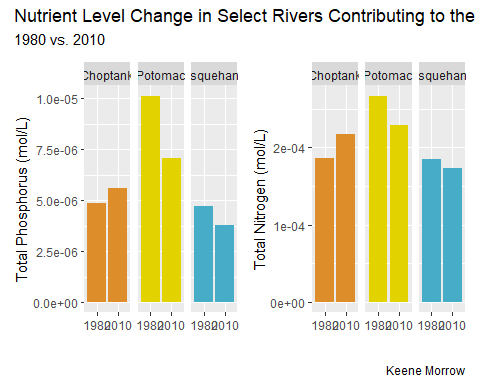
\includegraphics{esm202_hw1_MORROW_files/figure-latex/unnamed-chunk-20-1.pdf}

Between 1980 and 2010 the Potomac and Susquehanna Rivers saw reductions
in both total phosphorus and total nitrogen, with the greatest reduction
being in total phosphorus in the Potomac. By contrast, both total
phosphorus and total nitrogen increased in the Choptank River in the
same time period. This difference is liekly due to the Choptank's
contributing area being exclusively agricultural land versus the Potomac
being urban in addition to agricultural and the Susquehanna being
forested and rural in addition to agricultural. It is expected that the
princinpal source of excess nitrogen and phosphorus in the rivers is
agricultural runoff.

\end{document}
